\chapter{Results}
\label{section:7_Results}

This chapter presents a more accurate description of the results obtained in~\cref{section:Parameters_to_SXR} as they represents an actual implementation of most of the ML methods presented so far.
The structure that has been applied is the same reported in~\Figure{\ref{fig:SXR_from_param}} where a Variadic Autoencoder has been joined with a standard inference network to map the the magnetic configuration into the SXR latent space reconstruction, and than this latent configuration back to the SXR representation.

\subsection{Relevance layer}

The structure of the networks that have been used to construct these results starts from a \VAE{6} (autoencoder with a latent dimension of 6) and a inference network converting a generic feature from other sensors into that latent set.
These are the same structures that have been applied to obtain the previous results, but a further layer has been added to networks. Although based on a very simple idea, this layer is not coming from a standard ML methodology, so we decided to discuss it here. 

The idea comes from the observation that the at a certain point we needed to decide which plasma parameters had to be fed in the inference network to reconstruct the latent state. Obviously the selected parameters started from a guess of a sufficient information on the physical model that links the magnetic configuration to the temperature profile, even if in this case a complete mapping is not available.
% SPIEGARE QUI PERCHE'
In the limit of a reasonable number of inputs we decided to be create a rich set starting from some standard parameters, like the plasma current ($I_p$), toroidal loop potential ($V_t$), the reversal ($F$) and the ration of the dominant mode over secondaries ($NS$). Beside these a complete description, in argument and phase, of 15 modes from m=1 perturbation should provide the needed plasma shape to the network making it able to identify the position and the amplitude of the QSH.

However to define which are the most relevant parameters that play a role in the description of the plasma temperature we decided to turn the problem upside down. The idea indeed it to make the network itself yielding this from the training. Thus this layer is a simple dense perceptron where the linear pass through activation and an \textbf{identity matrix} for the weights. The point is that this is the former layer of the network, directly attached to the input features, and the weights are trainable. The layer definition needs also to constrain the initialization to set the identity and to fix all the other link to be kept to zero. 

Then during training the backpropagation tends to create a selection automatically by suppressing the inputs that are not contributing to the reduction of the loss, i.e. that does not correlate with the temperature profile.
So along the training epochs the loss, and possibly all the further regularization added, gradually silence that signals. This provides, not only a further layer that masks the non relevant inputs, bus once the weights are eventually exposed a short of "relevance" meter that can tell what inputs the target is more sensible at.
%
\begin{figure}
    \centering
    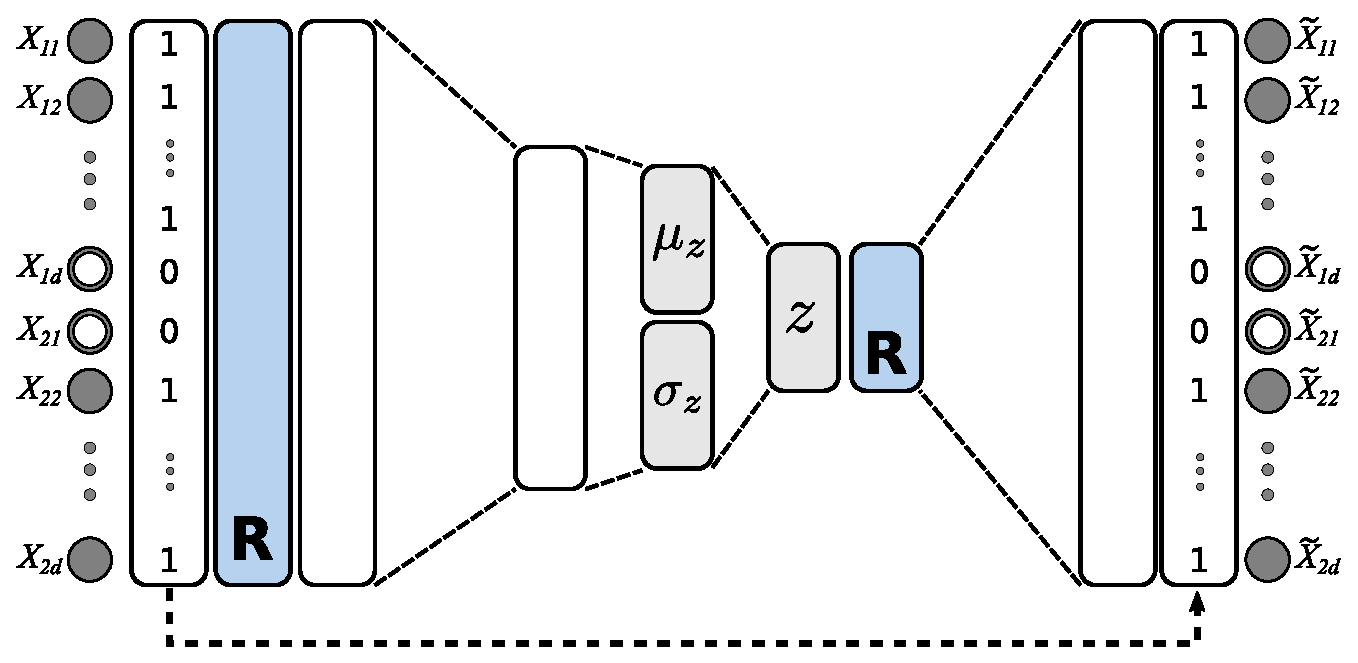
\includegraphics[height=6cm]{img/STEP12_7/VAE_RELEVANCE.eps}
    \caption{Relevance layer}
    \label{fig:relevance}
\end{figure}
%
The implemented idea is shown schematically in \Figure{\ref{fig:relevance}}, where the basic schema of a VAE with missing input is presented. The new relevance layers, shown with the (R) mark on the picture, can be placed after the input feature layer (just after the NaN-Mask layer) and/or at the latent space layer (the first layer of the decoder).
Although the picture shows the case of an Autoencoder, the same layer can be applied to a simple inference too.
In the case of the Autoencoder the first relevance layer will provide the amount of mutual information that each particular input has with the others, while the second will give a hint on how much the encoder is providing a disentangled representation because the redundant dimension are kept out from the generative process.
On the other hand the simple application on a standard regression network such the one that we used to pass from magnetics to the temperature profiles provides the actual significance of each input parameter to the task of building the guess.

A sparsity promotion regularizer, such as the dropout, beside the effects on the network generalization, shown to improve the relevance too.
In \Figure{\ref{fig:step_12_7_relevance}} the training process for the parameters inference is presented, togeteher with the obtained relevance values for all the inputs.
These results are not yet conclusive, however the expected dependence on the m=1 n=-7 argument is confirmed.
To obtain a more informative result a better use of regularization will be necessary possibly also characterizing the all values from a sequence of repeated training on the network.




For the implementation of the autoencoder a \VAE{6} has been used with only dense layers. We started from a input feature of 30 values that represent the 15 points of the temperature profiles. Then a encoder network 


\begin{figure}
    \centering
    \subfigure{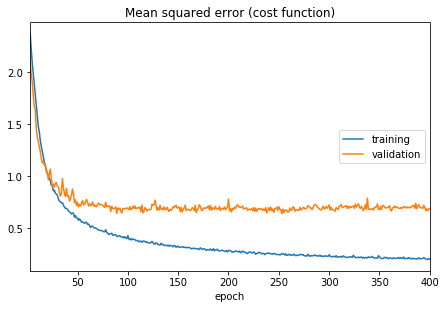
\includegraphics[height=3.3cm]{img/STEP12_7/STEP12_7_pBr2SXR_rm-rs_absarg_training_mse.png} \label{step_12_7_training}}
    \subfigure{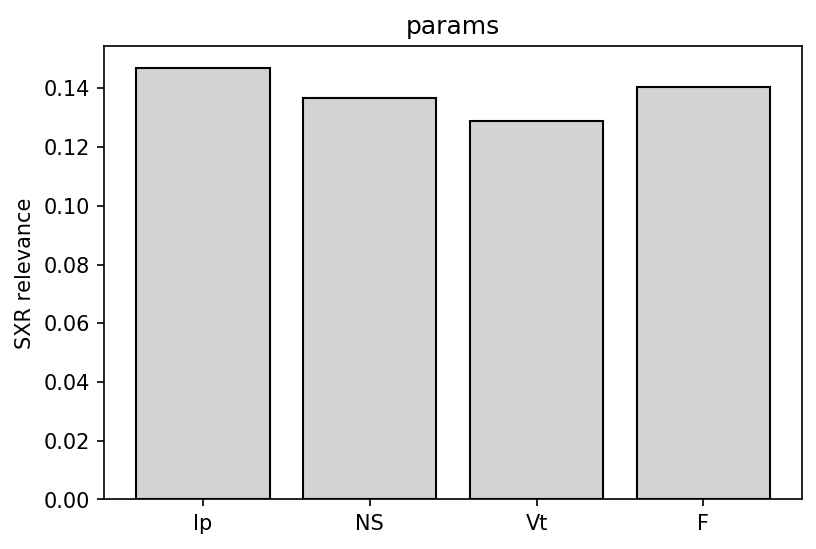
\includegraphics[height=3.3cm]{img/STEP12_7/STEP12_7_params.png} \label{step_12_7_p}}
    \subfigure{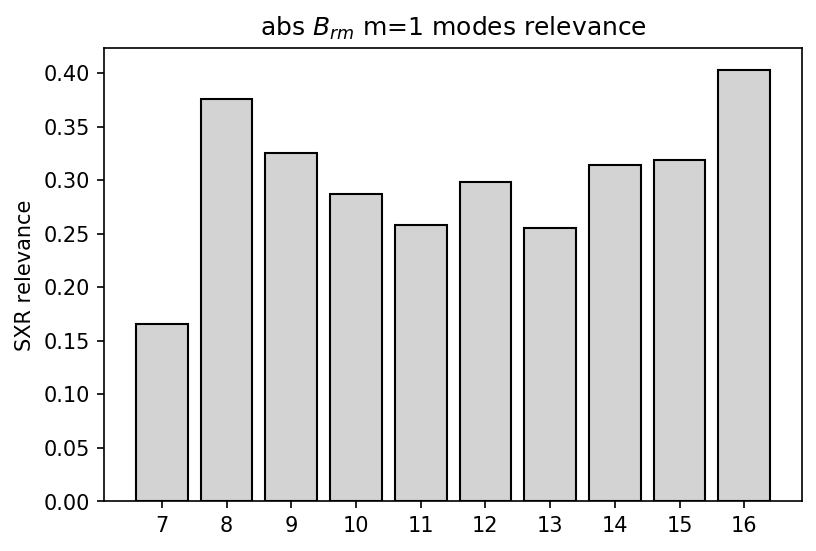
\includegraphics[height=3.3cm]{img/STEP12_7/STEP12_7_abs_Br_rm.png} \label{step_12_7_abs_Brm}}
    \subfigure{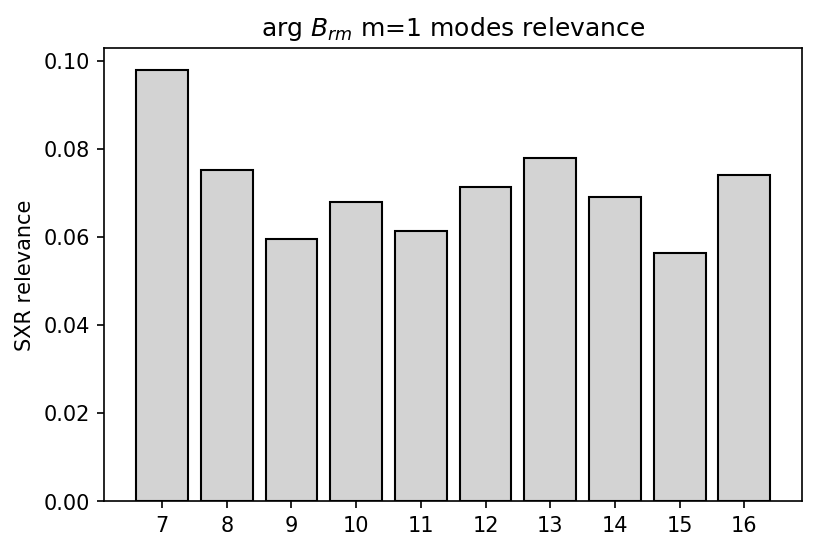
\includegraphics[height=3.3cm]{img/STEP12_7/STEP12_7_arg_Br_rm.png} \label{step_12_7_arg_Brm}}
    \subfigure{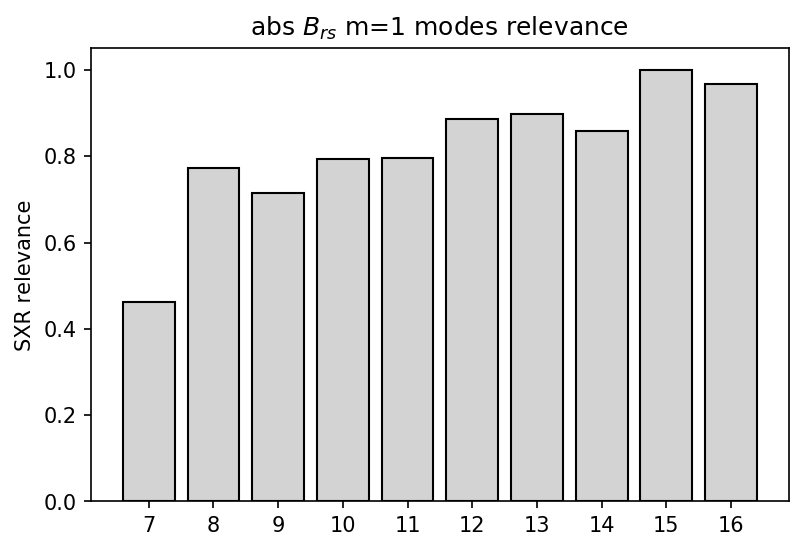
\includegraphics[height=3.3cm]{img/STEP12_7/STEP12_7_abs_Br_rs.png} \label{step_12_7_abs_Brs}}
    \subfigure{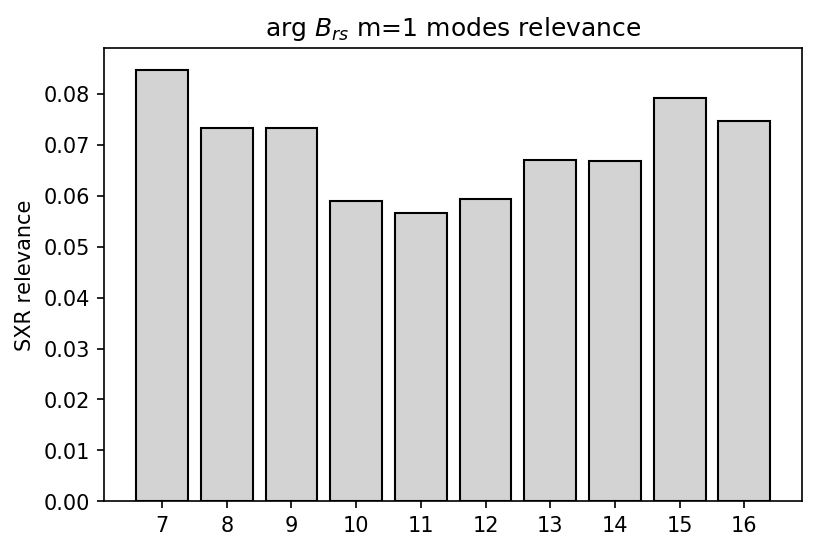
\includegraphics[height=3.3cm]{img/STEP12_7/STEP12_7_arg_Br_rs.png} \label{step_12_7_arg_Brs}}
    \caption{ Training 500 epochs - STEP 12.7 mse, slightly overfitted but validation not diverging }
    \label{fig:step_12_7_relevance}
\end{figure}


\begin{figure}
\centering

a.\subfigure{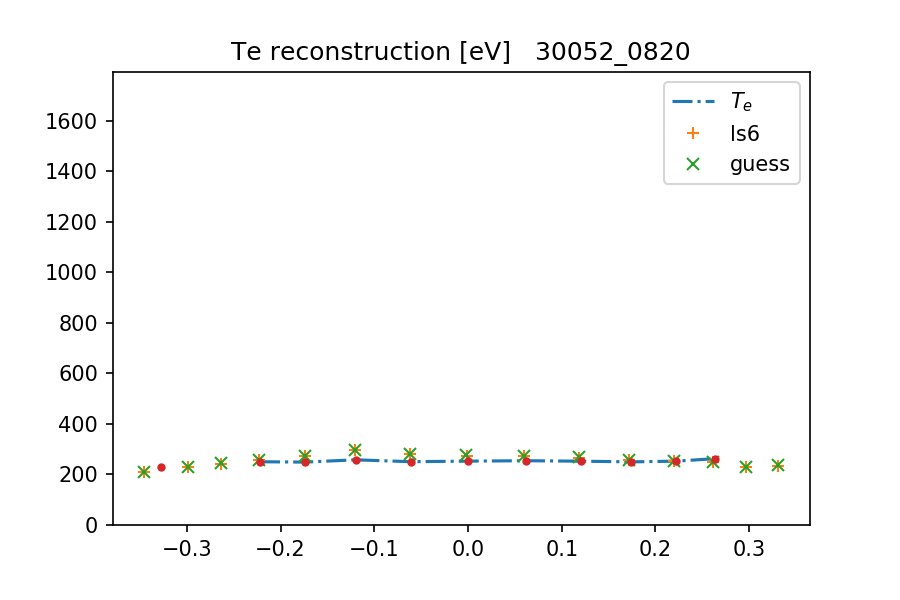
\includegraphics[height=4cm,trim={0.5cm 0cm 0.5cm 0.5cm},clip]{img/STEP12_7c/Te_rec_16.png}   }%    
\subfigure{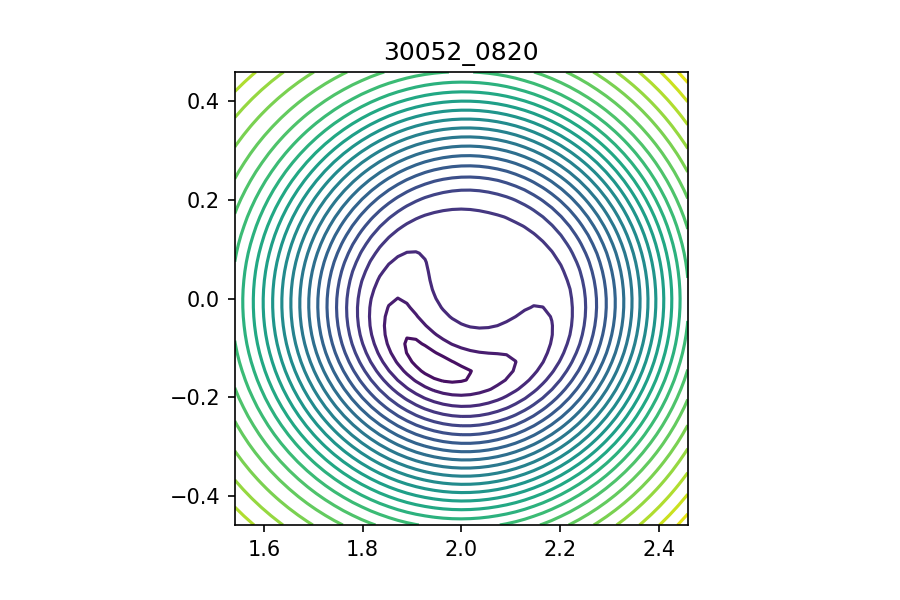
\includegraphics[height=4cm,trim={3cm   0   3.5cm 0    },clip]{img/STEP12_7c/Contour_16.png}  }%   
\subfigure{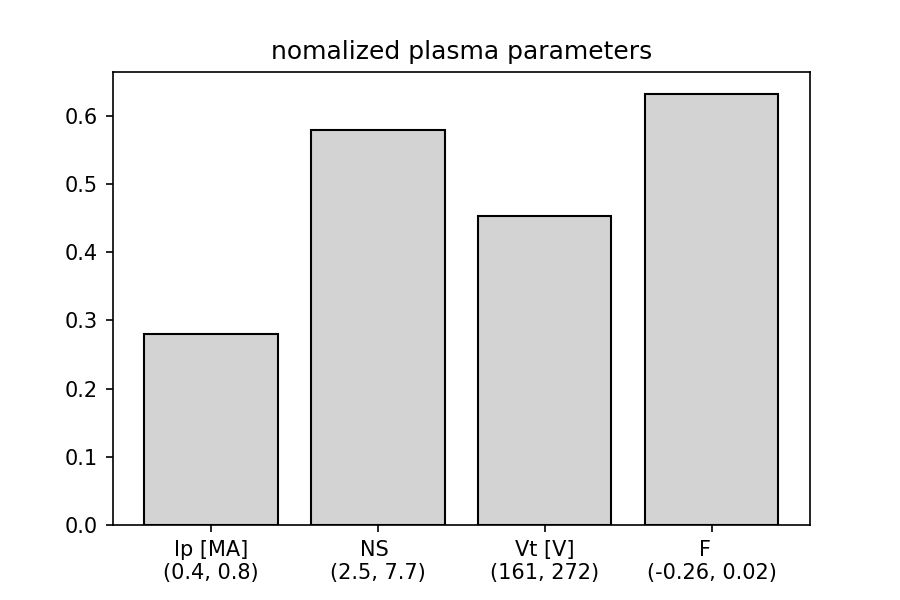
\includegraphics[height=4cm,trim={0.5cm 0cm 0.5cm 0cm  },clip]{img/STEP12_7c/Params_16.png}   }\\%
b.\subfigure{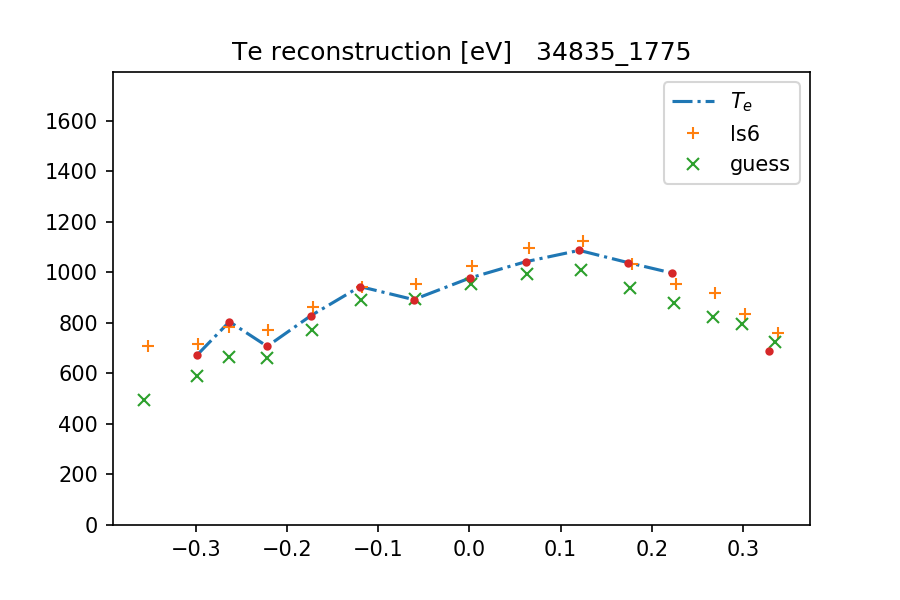
\includegraphics[height=4cm,trim={0.5cm 0cm 0.5cm 0.5cm},clip]{img/STEP12_7c/Te_rec_143.png}  }%   
\subfigure{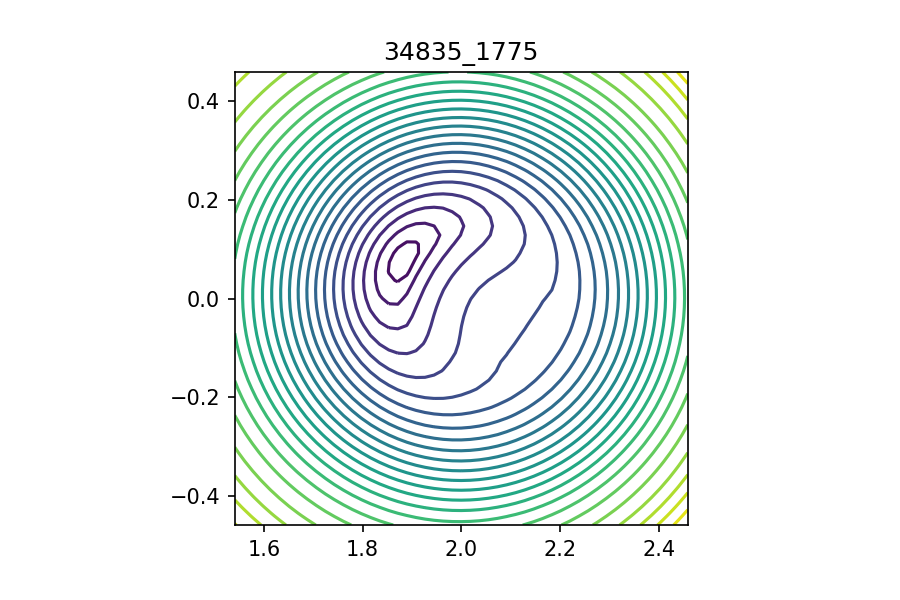
\includegraphics[height=4cm,trim={3cm   0   3.5cm 0    },clip]{img/STEP12_7c/Contour_143.png} }%  
\subfigure{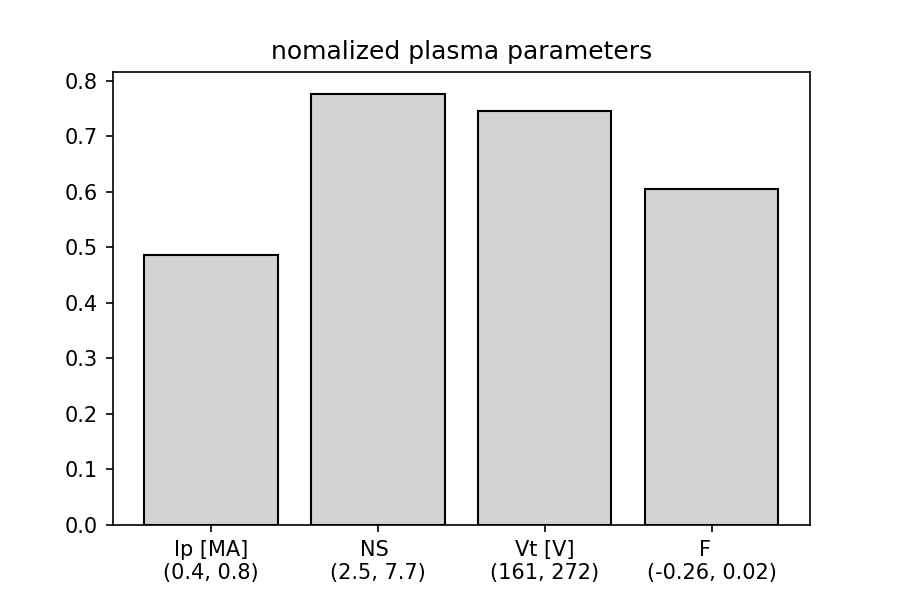
\includegraphics[height=4cm,trim={0.5cm 0cm 0.5cm 0cm  },clip]{img/STEP12_7c/Params_143.png}  }\\%
c.\subfigure{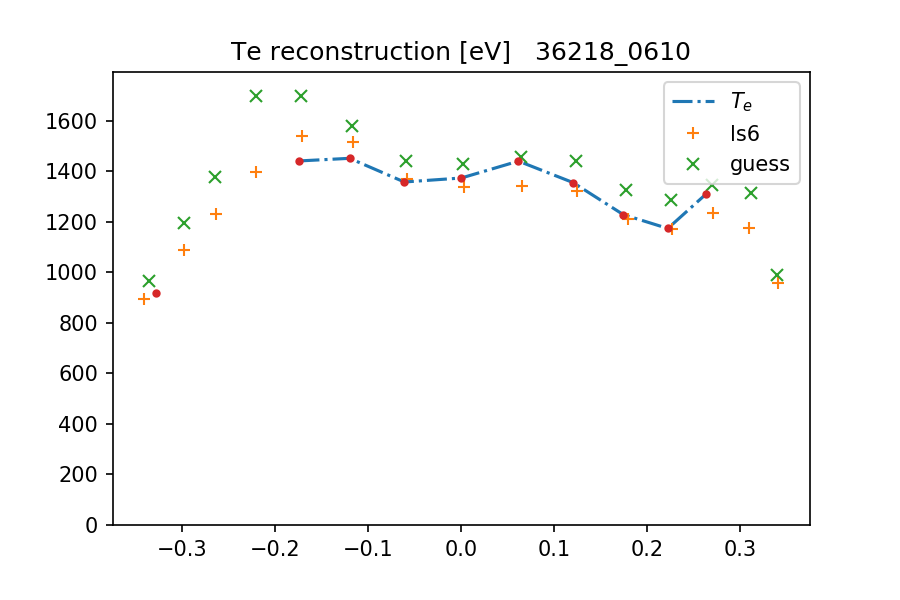
\includegraphics[height=4cm,trim={0.5cm 0cm 0.5cm 0.5cm},clip]{img/STEP12_7c/Te_rec_201.png}  }%   
\subfigure{\includegraphics[height=4cm,trim={3cm   0   3.5cm 0    },clip]{img/STEP12_7c/Contour_201.png} }%  
\subfigure{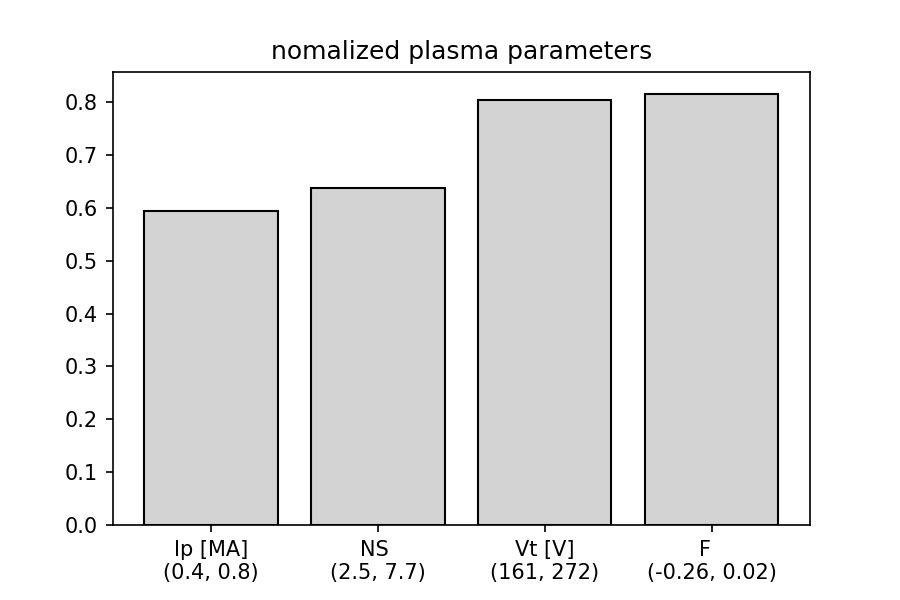
\includegraphics[height=4cm,trim={0.5cm 0cm 0.5cm 0cm  },clip]{img/STEP12_7c/Params_201.png}  }\\%
d.\subfigure{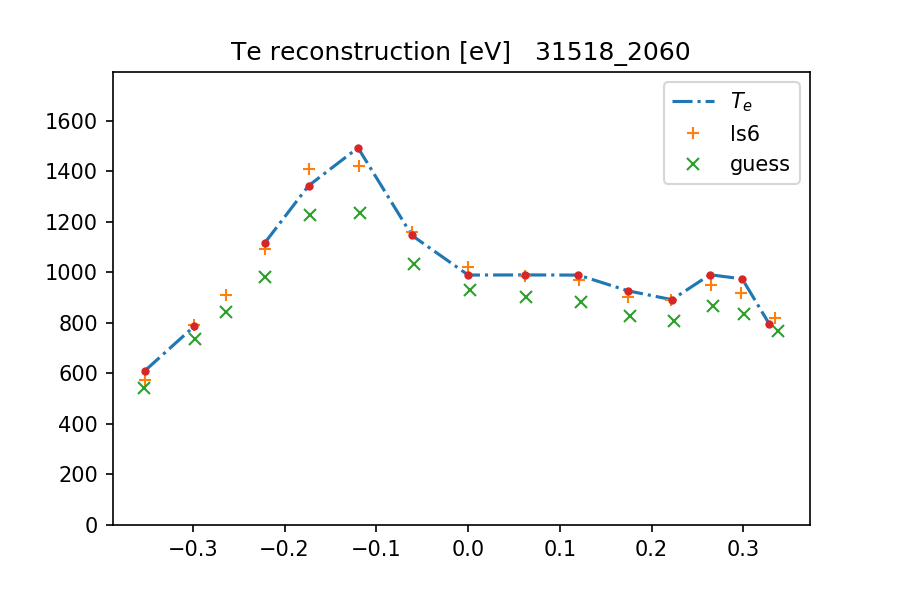
\includegraphics[height=4cm,trim={0.5cm 0cm 0.5cm 0.5cm},clip]{img/STEP12_7c/Te_rec_160.png}  }%   
\subfigure{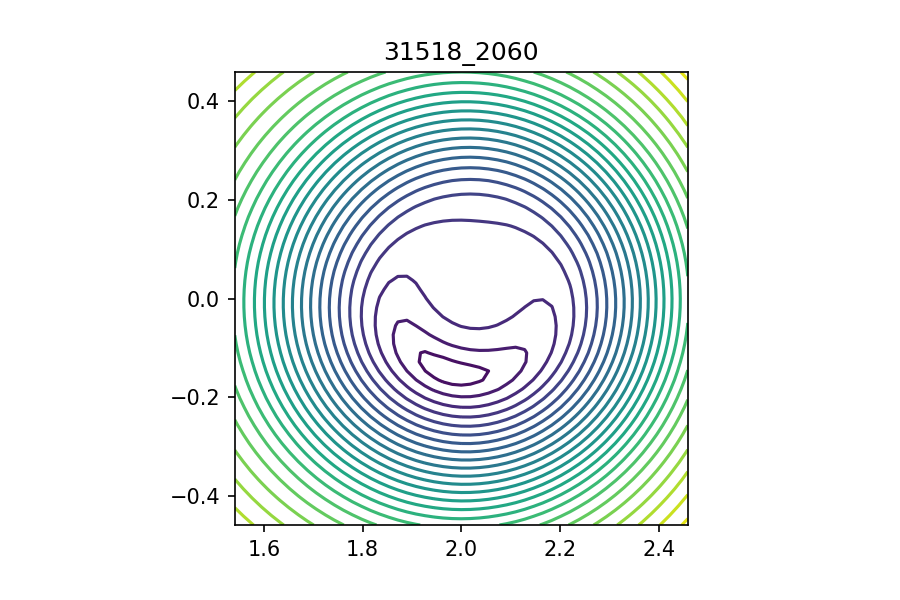
\includegraphics[height=4cm,trim={3cm   0   3.5cm 0    },clip]{img/STEP12_7c/Contour_160.png} }%  
\subfigure{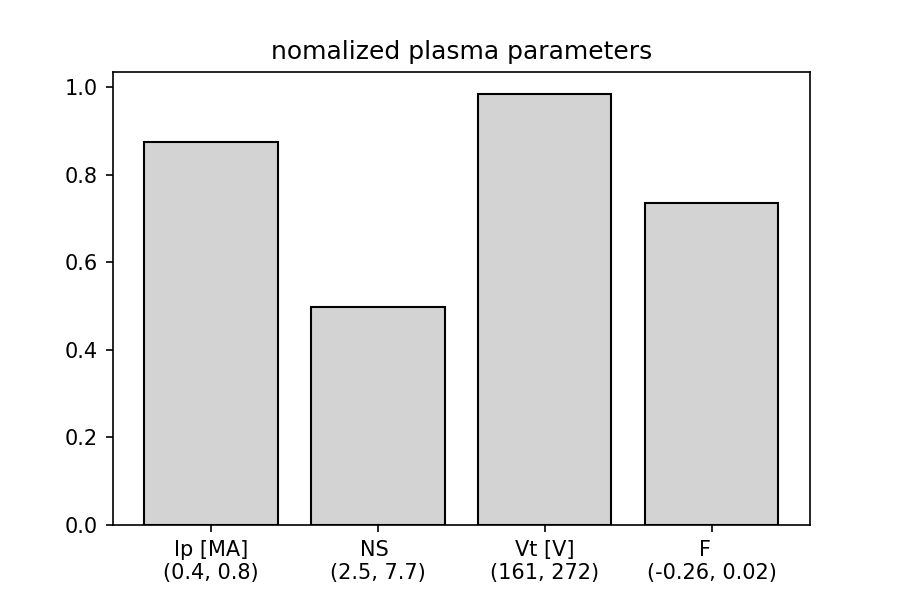
\includegraphics[height=4cm,trim={0.5cm 0cm 0.5cm 0cm  },clip]{img/STEP12_7c/Params_160.png}  }\\%
e.\subfigure{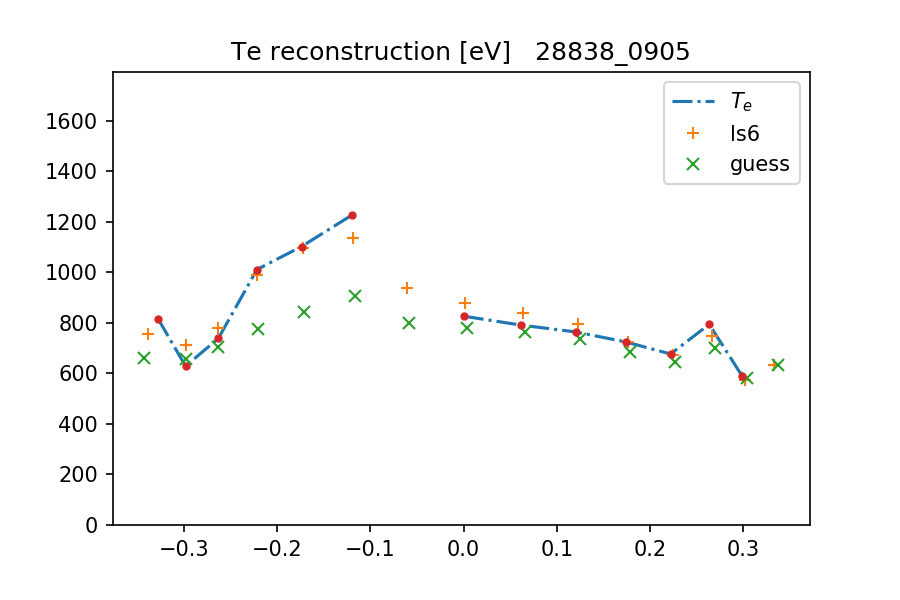
\includegraphics[height=4cm,trim={0.5cm 0cm 0.5cm 0.5cm},clip]{img/STEP12_7c/Te_rec_165.png}  }%   
\subfigure{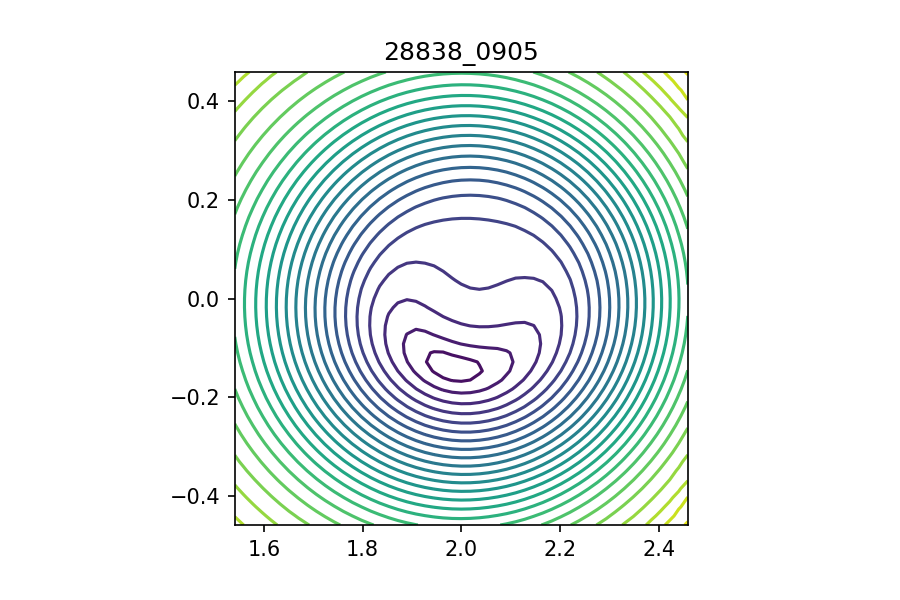
\includegraphics[height=4cm,trim={3cm   0   3.5cm 0    },clip]{img/STEP12_7c/Contour_165.png} }%  
\subfigure{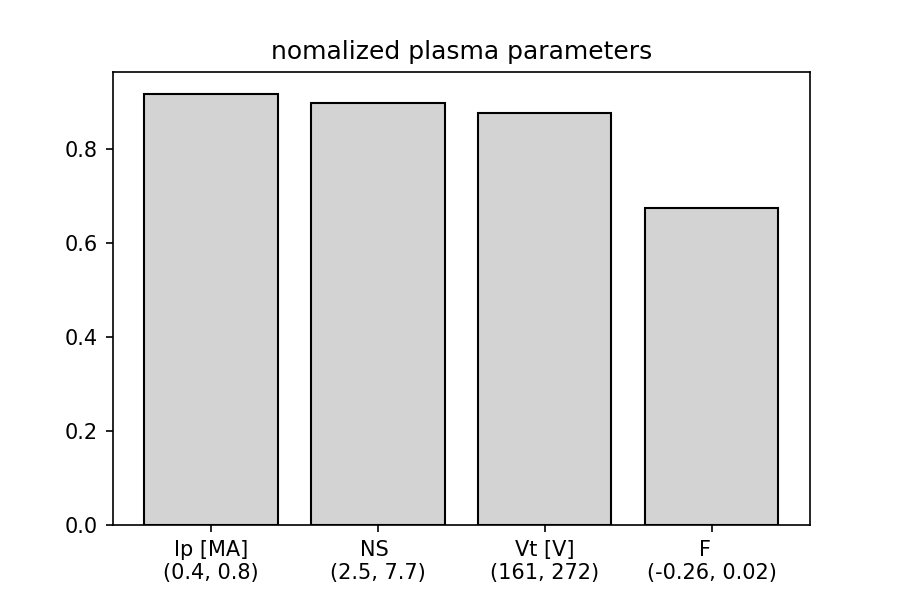
\includegraphics[height=4cm,trim={0.5cm 0cm 0.5cm 0cm  },clip]{img/STEP12_7c/Params_165.png}  }% 

% OLD
% \subfigure{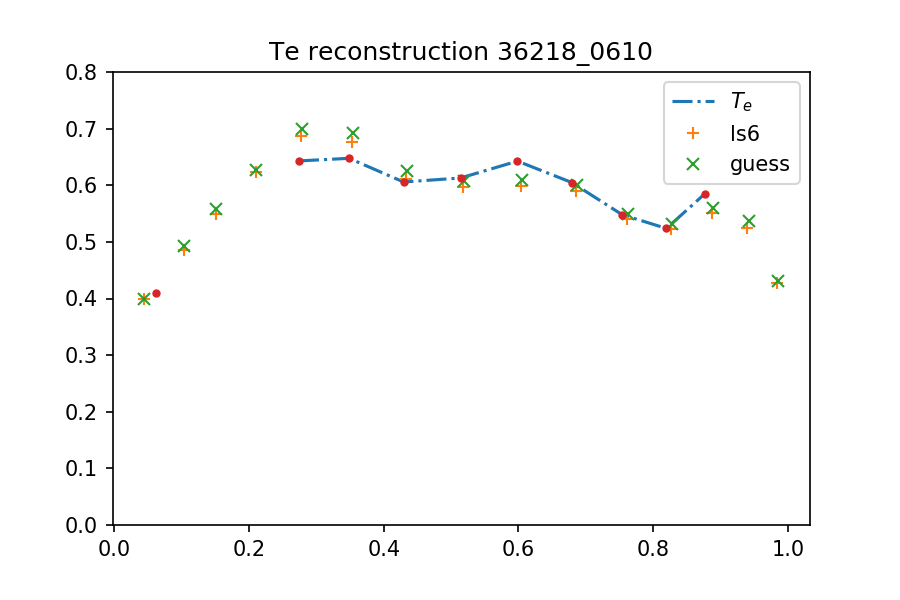
\includegraphics[height=4cm]{img/STEP12_7b/Te_rec_201.png}     }%
% \subfigure{\includegraphics[height=4cm]{img/STEP12_7b/Contour_201.png}    }%
% \subfigure{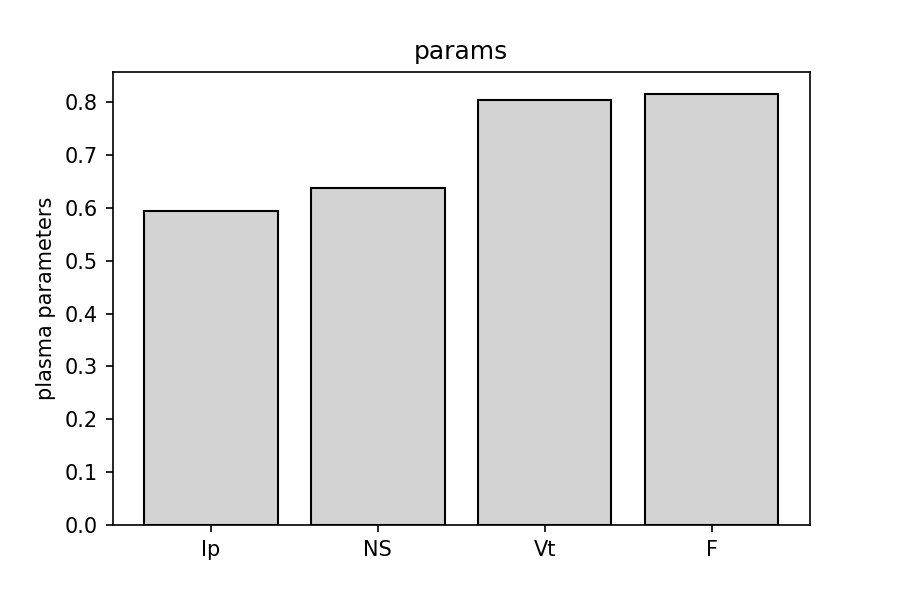
\includegraphics[height=4cm]{img/STEP12_7b/Params_201.png}     }\hfill
% \subfigure{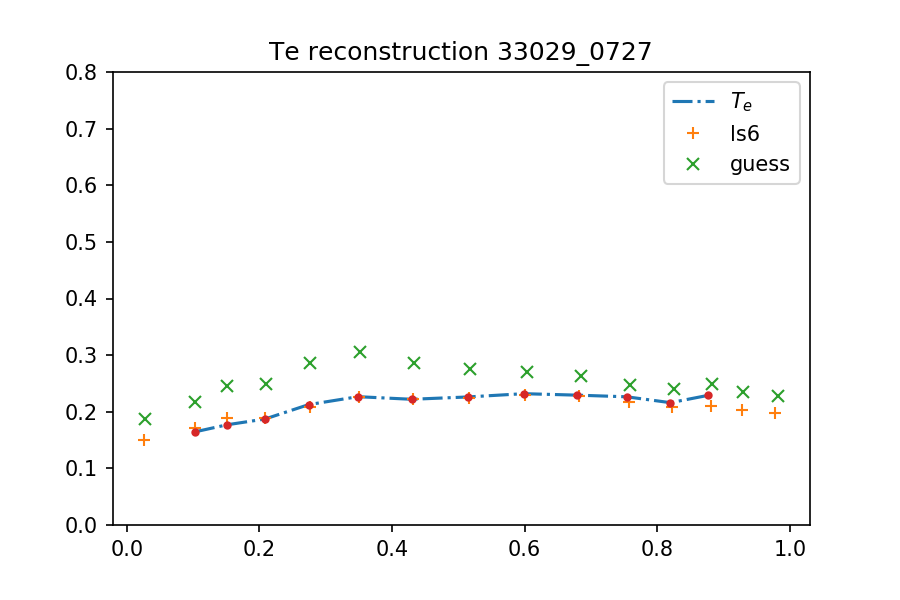
\includegraphics[height=4cm]{img/STEP12_7b/Te_rec_207.png}     }%
% \subfigure{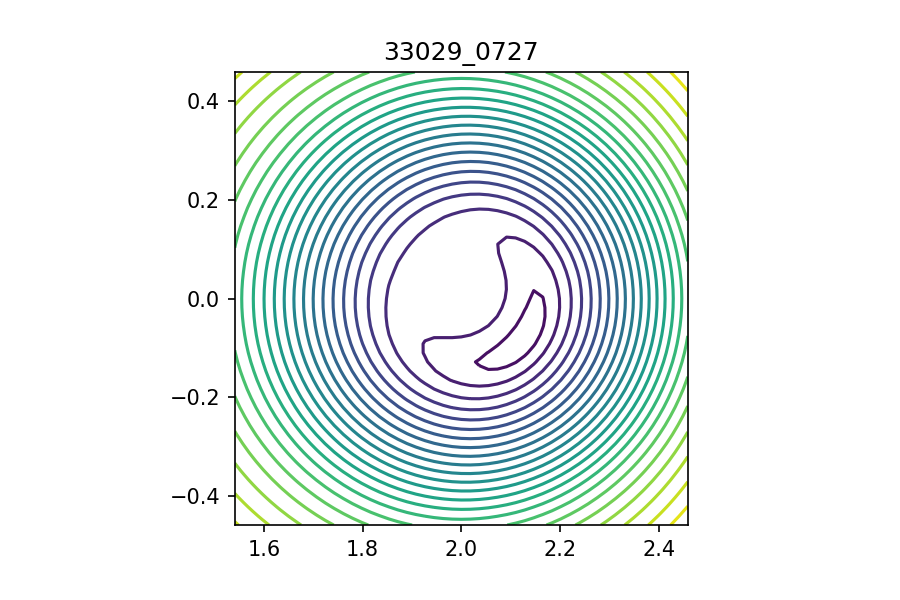
\includegraphics[height=4cm]{img/STEP12_7b/Contour_207.png}    }%
% \subfigure{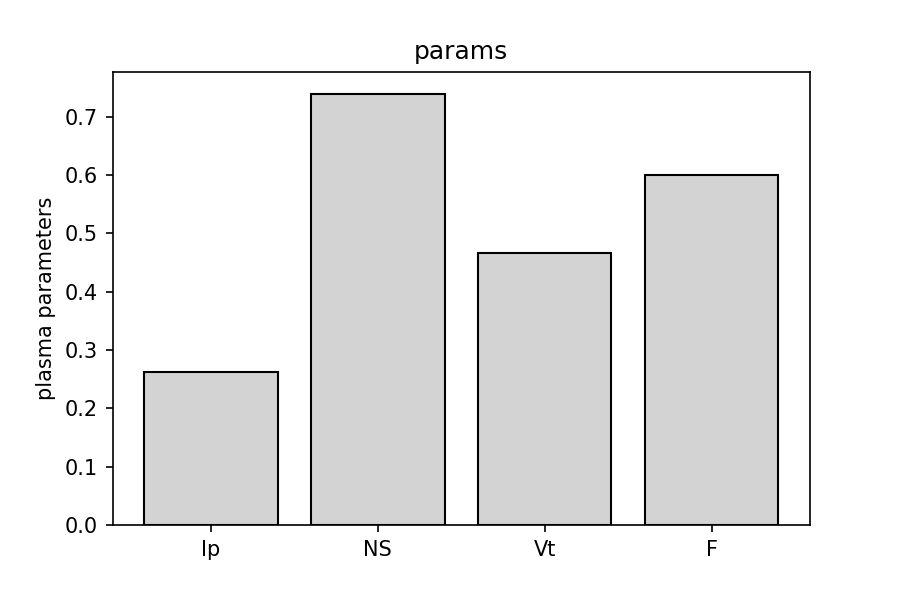
\includegraphics[height=4cm]{img/STEP12_7b/Params_207.png}     }\hfill
% \subfigure{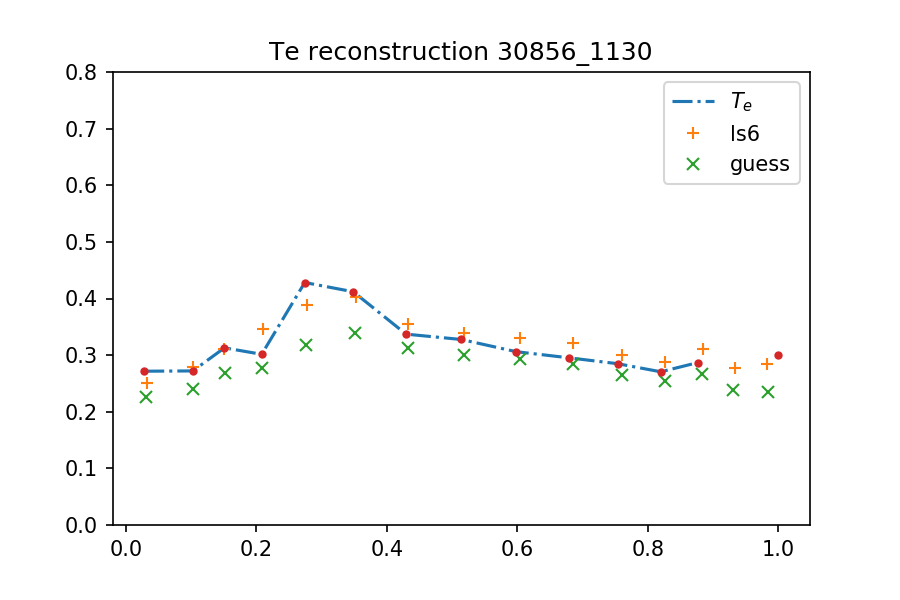
\includegraphics[height=4cm]{img/STEP12_7b/Te_rec_219.png}     }%
% \subfigure{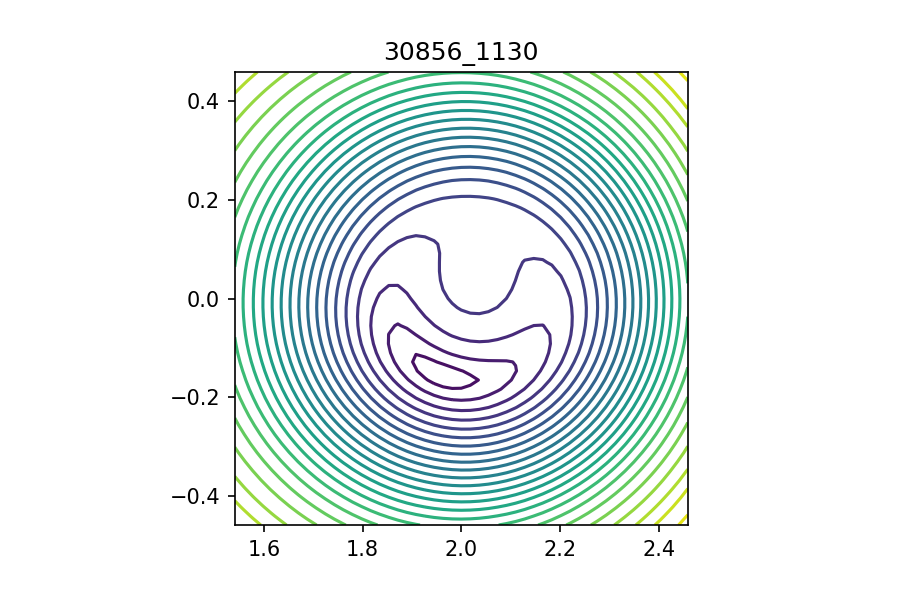
\includegraphics[height=4cm]{img/STEP12_7b/Contour_219.png}    }%
% \subfigure{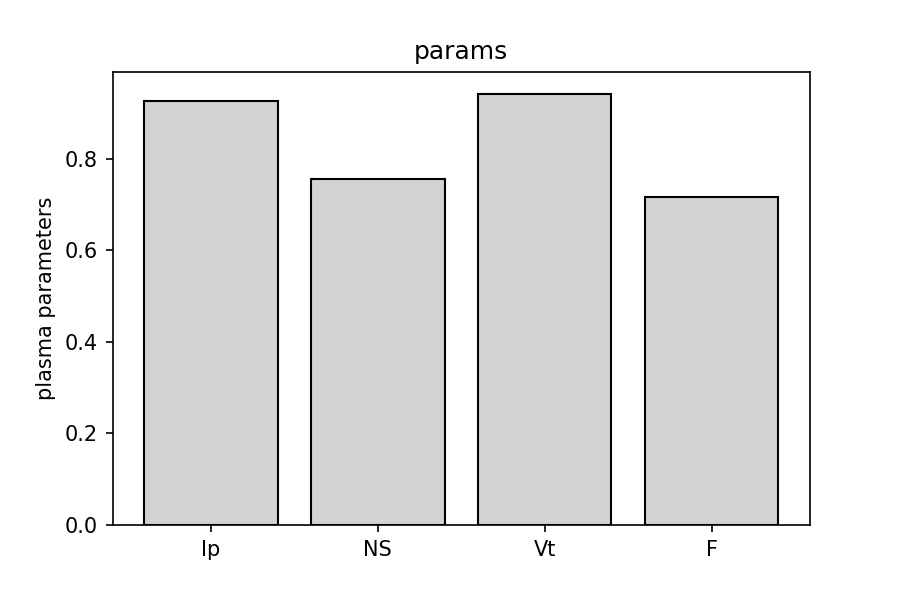
\includegraphics[height=4cm]{img/STEP12_7b/Params_219.png}     }\hfill
% \subfigure{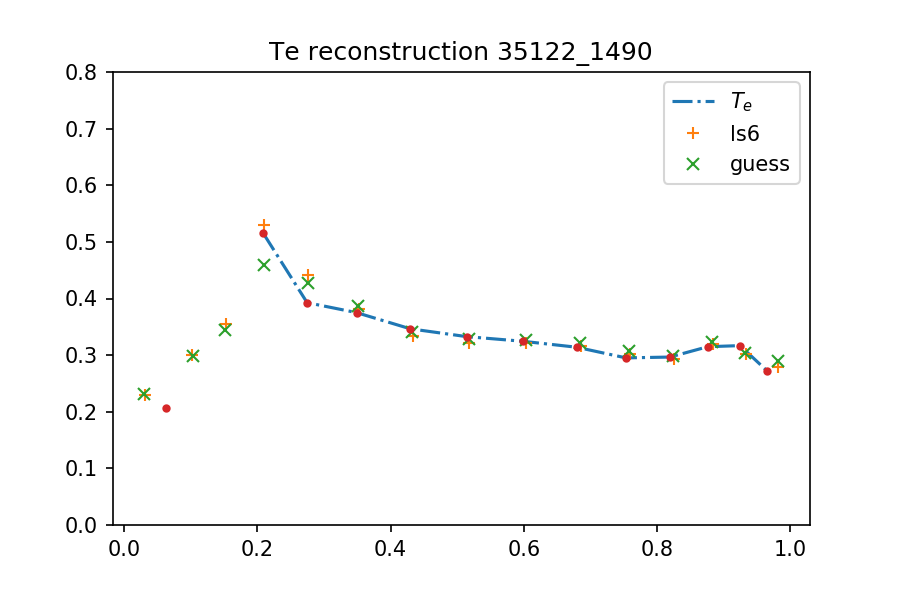
\includegraphics[height=4cm]{img/STEP12_7b/Te_rec_194.png}     }%
% \subfigure{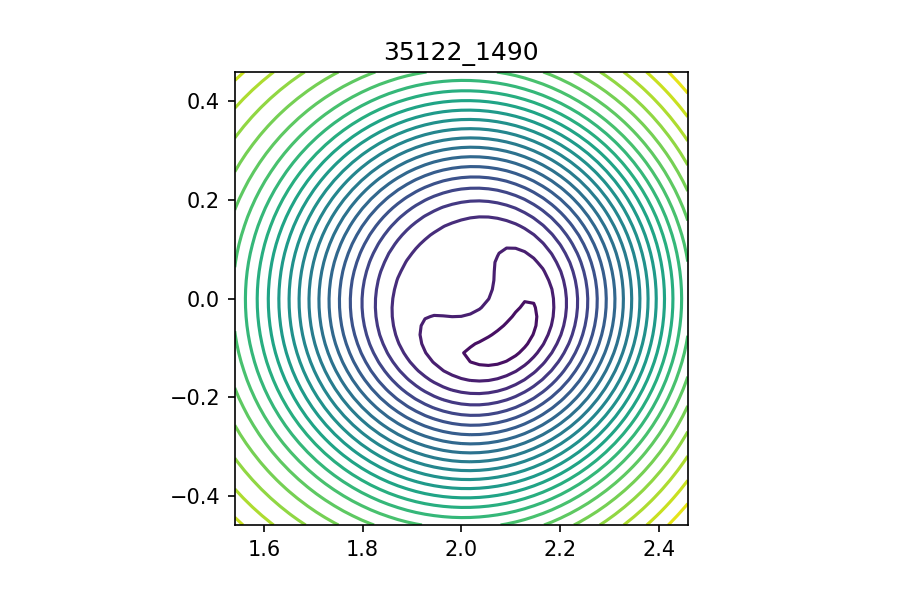
\includegraphics[height=4cm]{img/STEP12_7b/Contour_194.png}    }%
% \subfigure{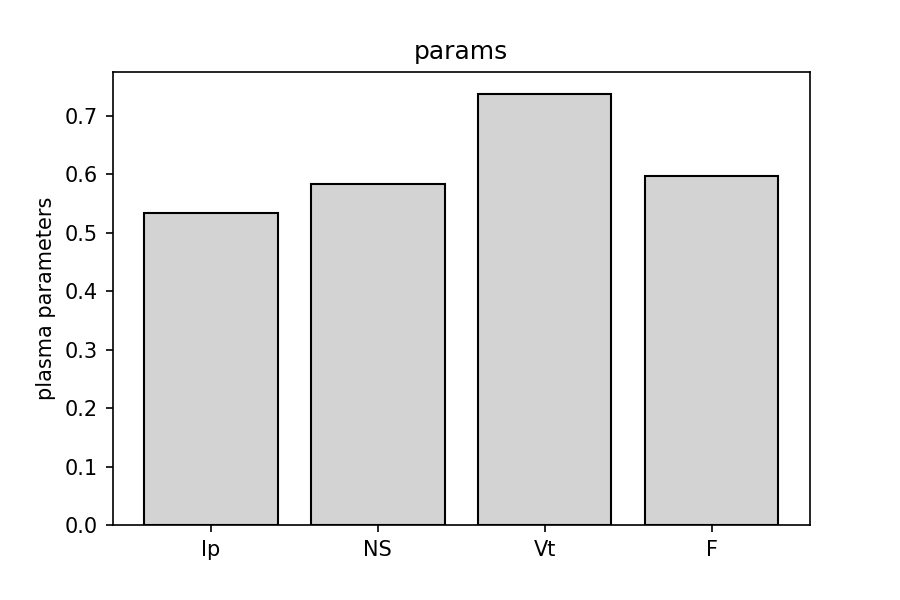
\includegraphics[height=4cm]{img/STEP12_7b/Params_194.png}     }\hfill

\caption{Reconstruction examples with plots of temperature profile, 2D reconstruction, and the related normalized plasma parameters. The temperature profile shows the real acquired $T_e$ from SXR3 with blue line (-.), the decoded profile from \VAE{6} in orange (+), and the inferred profile from magnetic configuration $(B_r, B_\varphi)$ at border. Three values of plasma current has been selected (a,b,c). A successful and failed phase identification is reported respectively in examples (d,e). }
\label{fig:Step_12_val}
\end{figure}




\begin{figure}
    \centering
    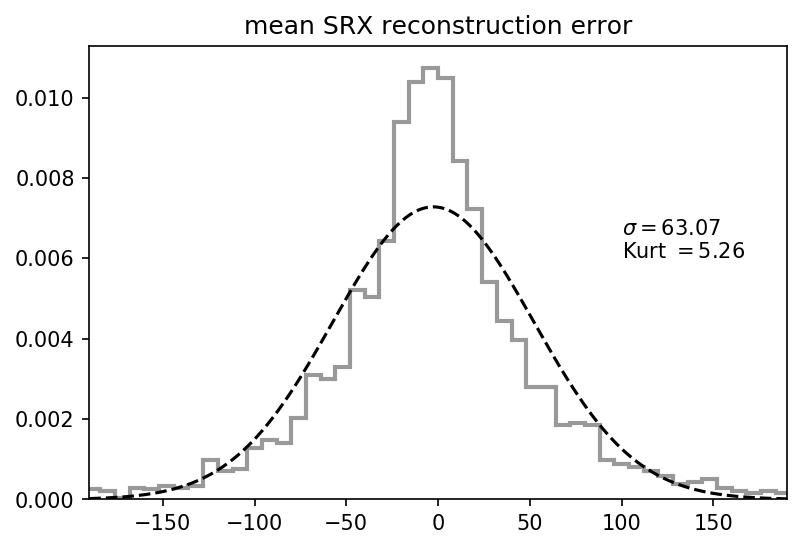
\includegraphics[height=6cm]{img/STEP12_7c/Mean_Absolute_Error.png}
    \caption{Mean absolute total reconstruction error for SXR profile inference from magnetic parameters. The distribution is obtained from the validation dataset and shows a standard deviation of 63 [eV]. }
    \label{fig:my_label}
\end{figure}


